\section{LeNet}
İlk olarak 1996 yılında Yann LeCun tarafından CNN bir makale şeklinde yayınlandı. 1998 yılında ilk uygulaması yine Yann LeCun ve ekibi tarafından posta numaraları, banka çekleri üzerindeki sayıların okunması için geliştirildi. Yann Lecun, ağın ismine "LeNet" adını vermiştir. MNIST veri seti üzerinde kullanılmıştır. Bu modelde boyut azaltma adımlarında max pooling yerine average pooling işlemi yapılmaktadır. Aktivasyon fonksiyonu olarak sigmoid ve hiperbolik tanjant kullanılmaktadır. Çıkışında softmax bulunmaktadır.

\begin{figure}[h]
    \centering
    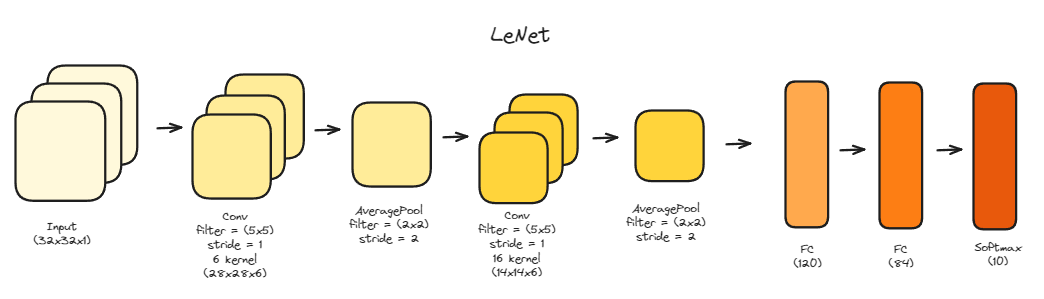
\includegraphics[width=1\textwidth]{images/lenet.png}
    \caption{LeNet mimarisi.}
    \label{fig:enter-label}
\end{figure}

\begin{lstlisting}[language=Python]
model = Sequential(
	# 32 - 5 / 1 + 1 = 28 -> 28x28x6
	Conv2D(6, 5, activation='tanh', input_shape=(28, 28, 1)),
	# (28x28x1) / (2x2) = (14x14x6)
	AveragePooling2D(2)),
	# 14 - 5 / 1 + 1 = 10 -> 10x10x16
	Conv2D(16, 5, activation='tanh')),
	# (10x10x16) / (2x2) = (5x5x16)
	AveragePooling2D(2)),

	# 120
	Flatten(),

	Dense(120, 5, activation='tanh')),
	Dense(84, activation='tanh')),
	Dense(10, activation='softmax'))
)
\end{lstlisting}

\newpage